\chapter{Background}
\label{ch:background}

This chapter introduces the foundational concepts underpinning this thesis.
Section~\ref{sec:bg-ai} provides a brief overview of artificial intelligence,
neural networks, and deep learning.
Section~\ref{sec:bg-workloads} formalizes DNN workloads and introduces the
extended Einsum notation used throughout this work.
Section~\ref{sec:bg-hw-accel} describes hardware acceleration for deep
learning and the abstraction of spatial architectures.
Section~\ref{sec:bg-mapping} defines the mapping problem and the degrees of
freedom available to a mapper.
Section~\ref{sec:bg-mapspace} analyzes the combinatorial explosion of the
resulting map-space.
Section~\ref{sec:bg-cost-model} discusses cost modeling for spatial
architectures.
Finally, Section~\ref{sec:bg-layer-fusion} introduces the concept of layer
fusion and its implications for memory traffic reduction.

% ------------------------------------------------------------------
% ============================================================
%  2.1  Artificial Intelligence
% ============================================================
\section{Artificial Intelligence}
\label{sec:bg-ai}

Throughout human history the aspiration to replicate human thought through
technology has been a persistent theme; written testimony of this desire dates
as far back as the II century B.C.E.\ in the myth of the bronze guardian Talos
and in its desire for immortality~\cite{talos}.
Talos furnishes the mythological foundation for the Greek concept of the
\emph{automaton}---an entity that moves of its own accord---and has been
invoked to illustrate the ability to solve problems autonomously, not through
the formal specification of rules, but by learning from experience which
choice is the most appropriate.

This inductive process, which enables the extraction of patterns from data,
is known as \emph{machine learning}.
As an inductive method, it is heavily dependent on the quantity and quality of
the data from which it learns, and in particular on the
\emph{representational form} of that data.
Initially, the selection of representations---called \emph{features}---had to
be performed manually by domain experts; this limitation was
subsequently overcome by \emph{deep learning},
in which complex concepts are represented hierarchically in terms of simpler
ones.
When visualized, this hierarchy of concepts forms a deep computational graph,
leading to the term \textbf{Deep Learning} (DL).
The fundamental principle of DL is to learn an efficient \emph{latent
representation} of the input data, one designed to capture the essential
semantic information required for a given task and to transform the problem
into a space where a solution can be more easily discovered.


% ------------------------------------------------------------
\subsection{The Perceptron}
\label{sec:perceptron}
% ------------------------------------------------------------

The cornerstone of modern neural networks is the \emph{perceptron}, the first
tangible implementation of an artificial learning neuron.
The concept was developed throughout the 1950s and 1960s by Frank
Rosenblatt~\cite{perceptron}, inspired by earlier work from Warren McCulloch
and Walter Pitts.

A perceptron takes several binary inputs, $x_1, x_2, \dots$, and produces a
single binary output.
Rosenblatt proposed a simple rule to compute this output by introducing
\textit{weights}, $w_1, w_2, \dots$, which are real numbers expressing the
relative importance of each input.
The neuron's output, either~$0$ or~$1$, is determined by whether the weighted
sum of its inputs, $\sum_j w_j x_j$, falls below or exceeds some
\textit{threshold value}.
Like the weights, the threshold is a real-valued parameter of the neuron.
This decision rule can be expressed algebraically as:
\begin{equation}
\label{eq:perceptron-threshold}
\text{output} = 
\begin{cases} 
0 & \text{if } \sum_j w_j x_j \le \text{threshold}, \\ 
1 & \text{if } \sum_j w_j x_j > \text{threshold}. 
\end{cases}
\end{equation}

To simplify the notation, two standard substitutions are made.
First, the summation is rewritten as a dot product,
$\mathbf{w} \cdot \mathbf{x} \equiv \sum_j w_j x_j$, where $\mathbf{w}$
and~$\mathbf{x}$ are vectors of the weights and inputs, respectively.
Second, the threshold is moved to the other side of the inequality and
replaced by the neuron's \textit{bias}, defined as
$b \equiv -\text{threshold}$.
The bias can be thought of as a measure of how easily the perceptron can be
made to output a~$1$, or, in biological terms, to ``fire.''
Using the bias, the perceptron rule becomes:
\begin{equation}
\label{eq:perceptron-bias}
\text{output} = 
\begin{cases} 
0 & \text{if } \mathbf{w} \cdot \mathbf{x} + b \le 0, \\ 
1 & \text{if } \mathbf{w} \cdot \mathbf{x} + b > 0. 
\end{cases}
\end{equation}

This mathematical model can be viewed as a simple decision-making unit that
evaluates and combines multiple pieces of evidence through weighted
contributions.
By tuning its weights and bias, the perceptron can be adapted to represent
various types of decision processes.
Its ability to \emph{learn} from data by iteratively adjusting these
parameters constitutes the key advancement over the McCulloch--Pitts (MP)
neuron model, which relied solely on fixed, hand-designed weights and
thresholds.


% ------------------------------------------------------------
\subsection{Neural Networks and Activation Functions}
\label{sec:neural-networks}
% ------------------------------------------------------------

While a single perceptron can weigh evidence to make a simple (linear)
decision, its power is amplified when multiple perceptrons are organized into
a \emph{network} of layers.
In such a network, the first layer makes decisions based on the raw
input evidence.
The outputs of this layer are then fed as inputs to a second layer, which can,
in turn, make decisions at a more complex and abstract level.
By stacking multiple layers, the network can engage in highly sophisticated
decision-making.

From an abstract perspective, a neural network can be represented as a
directed acyclic graph composed of interconnected nodes---or
\emph{neurons}---inspired by their biological counterparts.
Each neuron receives a set of input signals, each associated with a
specific weight, and produces an output signal as a learned response.
The graph structure enables data propagation from input neurons to output
neurons through a series of weighted connections that modulate signal
strength at each stage.

\paragraph{Activation functions.}
Despite its foundational importance, the perceptron as presented in
Section~\ref{sec:perceptron} is a purely linear classifier: its decision
boundary is always a hyperplane, which limits it to solving only
\emph{linearly separable} problems.
This critical shortcoming motivated the introduction of \emph{activation
functions}---non-linear transformations applied to the weighted sum before
producing the neuron's output.

Formally, a modern neuron computes:
\begin{equation}
\label{eq:neuron-activation}
a = f\!\bigl(\mathbf{w} \cdot \mathbf{x} + b\bigr),
\end{equation}
where $f(\cdot)$ is a non-linear activation function and $a$ is the neuron's
\emph{activation}, which is subsequently transmitted to other neurons in the
network. 
One of the earliest replacements for the perceptron's step function was the
\emph{sigmoid} function:
\begin{equation}
\label{eq:sigmoid}
\sigma(z) = \frac{1}{1 + e^{-z}},
\end{equation}
which maps any real-valued input to the interval $(0,\,1)$ and is smooth
everywhere, enabling gradient-based learning algorithms such as
backpropagation~\cite{backprop}.

In modern practice, the \emph{Rectified Linear Unit}
(ReLU)~\cite{relu_glorot} is the most widely used activation function:
\begin{equation}
\label{eq:relu}
\text{ReLU}(z) = \max(0,\,z).
\end{equation}
Although piecewise linear, ReLU introduces non-linearity at the origin and
has proven to train faster than smooth alternatives on deep architectures
due to its non-saturating gradient for $z > 0$.

The insertion of a non-linear activation function after each neuron's
linear operation is what grants multi-layer networks their expressive power.
Without it, any composition of linear functions would itself remain
linear, and adding layers would provide no additional representational
capacity.
With non-linearity, each successive layer can build on the features
identified by the previous one to model increasingly complex patterns.


% ------------------------------------------------------------
\subsection{Deep Neural Networks}
\label{sec:dnn}
% ------------------------------------------------------------

When a neural network is constructed with a substantial number of layers
stacked sequentially, it is referred to as a \textbf{Deep Neural Network}
(DNN).
This ``depth'' allows the network to learn a hierarchical representation
of data: early layers extract low-level features (such as edges or textures
in images), while deeper layers compose them into higher-level abstractions
(such as objects or semantic concepts).

Computationally, each neuron in a DNN performs a weighted summation of its
inputs---an operation that primarily consists of \emph{multiply-accumulate}
(MAC) computations---followed by the application of an activation function.
The output activation is then transmitted to connected neurons in the next
layer, often in a multicast manner.
In practice, DNNs are composed of various types of specialized
layers, each implementing a specific mathematical function or
\emph{computational kernel}; due to the sheer number of
MAC operations involved and the volume of data they process,
their efficient execution has become a first-class engineering challenge,
as will be discussed in Section~\ref{sec:bg-hw-accel}.

\paragraph{Scope of this work.}
This thesis focuses exclusively on DNN \emph{inference}---the forward
evaluation of a trained model on new inputs---rather than on training, 
which involves the additional computation of gradients and parameter
updates through backpropagation.
While training workloads impose their own distinct hardware demands,
the computational kernels executed during inference (predominantly
convolutions and matrix multiplications) are the same as those in the
forward pass of training, making the analytical framework developed in
this work broadly applicable.
   % 2.1  Artificial Intelligence
% ------------------------------------------------------------------
% ============================================================
%  2.2  DNN Workloads and Notation
% ============================================================
\section{DNN Workloads and Notation}
\label{sec:bg-workloads}

Having established what a DNN is in Section~\ref{sec:bg-ai}, we now turn to
formalizing the \emph{computational workload} that each layer imposes on
hardware.
This formalization is essential because the mapping problem---how to schedule
and tile a workload onto a spatial architecture---is defined entirely in
terms of the loop-nest structure derived from it.


% ------------------------------------------------------------
\subsection{A Layer as a Loop Nest}
\label{sec:loop-nest}
% ------------------------------------------------------------

Every DNN layer can be decomposed into one or more
\emph{multiply-accumulate} (MAC) operations applied to three tensors:
an \emph{input activation} tensor, a \emph{weight} (or filter) tensor,
and an \emph{output activation} tensor.
A bias term, when present, is absorbed into the output initialization and
does not affect the loop-nest structure.

Because the MAC is associative and commutative, the order in which the
individual multiplications and accumulations are carried out is
irrelevant to the final numerical result.
This observation is crucial: it means the computation can be expressed as
a set of perfectly nested loops iterating over the various tensor
dimensions, and one is free to tile, reorder, and parallelize these loops
without altering correctness.

\paragraph{Example: one-dimensional convolution.}
To make the discussion concrete, consider a 1D convolution that maps an
input with $C$ channels and spatial extent $H$ to an output with $M$
channels and spatial extent $P$, using filters of size $R$:
\begin{equation}
\label{eq:1dconv}
\texttt{Output}[m,\, p] \;=\; \sum_{c=0}^{C-1}\;\sum_{r=0}^{R-1}
  \texttt{Input}[c,\, p{+}r]\;\times\;\texttt{Filter}[m,\, c,\, r],
\end{equation}
where $m \in [0,\,M)$ and $p \in [0,\,P)$.
Each output element requires $C \times R$ MAC operations, and the total
work is $M \times P \times C \times R$ MACs.

This expression can be read directly as a four-deep loop nest:

\begin{center}
\begin{minipage}{0.55\textwidth}
\begin{verbatim}
  for m in [0, M):
    for p in [0, P):
      for c in [0, C):
        for r in [0, R):
          Out[m][p] += W[m][c][r] * In[c][p+r]
\end{verbatim}
\end{minipage}
\end{center}

\noindent
The four loop dimensions---$M$, $P$, $C$, $R$---constitute the
\emph{iteration space} of the computation.
The key property is that these loops can be freely reordered (all $4!$
permutations produce the same output) and each loop can be tiled
(split into an outer and an inner sub-loop) to create smaller sub-problems
that fit in limited on-chip memories.
This flexibility is the foundation of all mapping strategies discussed in
Section~\ref{sec:bg-mapping}.

\paragraph{Extension to 2D convolutions.}
The standard 2D convolution, as used in CNNs, adds a second spatial
dimension and a batch dimension, leading to a seven-deep loop nest:
\begin{equation}
\label{eq:2dconv}
\texttt{O}[n,\,m,\,p,\,q]
  = \sum_{c}\;\sum_{r}\;\sum_{s}
    \texttt{I}[n,\,c,\,p{+}r,\,q{+}s] \;\times\;
    \texttt{W}[m,\,c,\,r,\,s],
\end{equation}
with dimensions $N$ (batch), $M$ (output channels), $P$ and $Q$ (output
spatial), $C$ (input channels), and $R$, $S$ (filter spatial).
This is the most common single-layer workload targeted by DNN accelerators
and the one used in the experimental evaluation of this thesis.


% ------------------------------------------------------------
\subsection{Coupling: the Relationship Between Dimensions and Tensors}
\label{sec:coupling}
% ------------------------------------------------------------

Each loop dimension in the nest participates in the indexing of one or
more of the three operand tensors.
The precise binding between dimensions and tensors---which we call the
\emph{coupling}---fully determines what data each iteration reads and
writes, and therefore what reuse opportunities exist.

\begin{definition}[Coupled and orthogonal dimensions]
\label{def:coupled-orthogonal}
A dimension $d$ is said to be \textbf{coupled} to an operand if $d$
appears in that operand's index expression (i.e., changing $d$ changes
the element accessed).
Conversely, $d$ is \textbf{orthogonal} to an operand if $d$ does not
appear in any of its index expressions; the operand's tile remains
constant as $d$ iterates, enabling complete \emph{stationarity} of that
operand.
\end{definition}

Consider the 2D convolution of Eq.~\eqref{eq:2dconv}.
Table~\ref{tab:coupling-conv} shows the coupling for each operand.
Every dimension is coupled to exactly two of the three operands and
orthogonal to one, creating a clean three-way partition that directly
maps onto the classical stationary dataflows (weight-stationary,
input-stationary, output-stationary), as discussed in
Section~\ref{sec:bg-mapping}.

\begin{table}[htbp]
\centering
\caption{Coupling of the standard 2D convolution.
A \checkmark\ indicates the dimension is coupled to (indexes) the operand;
a -- indicates orthogonality.}
\label{tab:coupling-conv}
\smallskip
\begin{tabular}{lccc}
\toprule
\textbf{Dimension} & \textbf{Input} & \textbf{Weight} & \textbf{Output} \\
\midrule
$M$ (out channels)   & --             & \checkmark      & \checkmark \\
$C$ (in channels)    & \checkmark     & \checkmark      & -- \\
$R$ (filter height)  & \checkmark     & \checkmark      & -- \\
$S$ (filter width)   & \checkmark     & \checkmark      & -- \\
$P$ (out height)     & \checkmark     & --              & \checkmark \\
$Q$ (out width)      & \checkmark     & --              & \checkmark \\
$N$ (batch)          & \checkmark     & --              & \checkmark \\
\bottomrule
\end{tabular}
\end{table}


% ------------------------------------------------------------
\subsection{Normal and Affine Dimensions}
\label{sec:normal-affine}
% ------------------------------------------------------------

Not all loop dimensions interact with tensor indices in the same way.
We distinguish two fundamental categories:

\begin{definition}[Normal dimension]
\label{def:normal-dim}
A dimension $d$ is \textbf{normal} if it appears alone as a tensor index
for every operand it is coupled to.
A normal dimension indexes each coupled operand independently: changing
$d$ selects a completely \emph{different} element along that operand's
corresponding axis.
\end{definition}

\begin{definition}[Affine dimension]
\label{def:affine-dim}
A dimension $d$ is \textbf{affine} if, for at least one operand, it
participates in a \emph{sum of indices} used to access a tensor
dimension.
That is, the operand is indexed by an expression of the form
$\alpha\, d + \beta \,d'$ (more generally, an affine combination of
two or more loop variables), rather than by $d$ alone.
\end{definition}

\paragraph{Illustration.}
In the 2D convolution of Eq.~\eqref{eq:2dconv}, the input
is indexed along its height by $p + r$.
Therefore:
\begin{itemize}
  \item $M$ and $C$ are \textbf{normal} dimensions: $M$ alone
    indexes the weight and output channel axes, $C$ alone indexes the
    input and weight channel axes.
  \item $R$ is \textbf{affine}: it appears in the sum $p + r$ that
    indexes the input's height.
    Likewise $S$ is affine via $q + s$.
  \item $P$ is also \textbf{affine}: it appears in the same sum $p + r$.
    $Q$ is affine via $q + s$.
\end{itemize}

The normal/affine distinction has deep consequences for mapping:
\begin{enumerate}
  \item \textbf{Tile-size computation.}
    When a normal dimension $d$ is tiled to size $t_d$ at some level, the
    operand tile along that axis is exactly $t_d$ elements.
    For an affine pair such as $(P,\,R)$, the input tile along the
    corresponding spatial axis is $t_P + t_R - 1$ (assuming unit stride),
    because consecutive output tiles \emph{overlap} in their input
    requirements.
  \item \textbf{Halo reuse.}
    When the innermost iterated dimension at a memory level is affine for
    an operand, consecutive iterations produce overlapping input tiles.
    Only the non-overlapping slice---the \emph{halo}---needs to be
    refetched, while the remaining data is reused from the previous
    iteration.
    This \emph{halo reuse} is unique to affine dimensions and does not
    arise with normal ones.
  \item \textbf{Map-space counting.}
    Only normal dimensions contribute independent tiling factors to the
    map-space cardinality (see Section~\ref{sec:bg-mapspace}).
    Affine dimensions affect tile sizes but are not independently looped;
    their tile sizes are derived from those of the normal dimensions
    they are summed with.
\end{enumerate}


% ------------------------------------------------------------
\subsection{Extended Einsum Notation}
\label{sec:een}
% ------------------------------------------------------------

To express the structure of tensor computations more concisely,
this thesis adopts the \textbf{extended Einsum notation}
(EEN)~\cite{abdelfattah2016EEN}, which augments the standard Einstein
summation convention with three features particularly suited to DNN
workloads:
\begin{enumerate}
  \item \textbf{Named ranks.}
    Each tensor dimension is given an explicit name (uppercase letter),
    and the variable iterating over it is denoted by the corresponding
    lowercase letter.
  \item \textbf{Shape tags.}
    Superscripts on each tensor specify the size of every rank, making
    the shapes explicit in the notation.
  \item \textbf{Affine subscripts.}
    Index expressions may contain sums of variables (e.g., $p + r$),
    directly encoding sliding-window and strided access patterns.
\end{enumerate}

Using the extended Einsum notation, the 1D convolution from
Eq.~\eqref{eq:1dconv} can be rewritten as:
\begin{equation}
\label{eq:een-1dconv}
\mathrm{Output}^{M,\,P}_{m,\,p}
  \;=\; \sum_{c,\,r}\;
  \mathrm{Input}^{C,\,H}_{c,\,p+r} \;\times\;
  \mathrm{Filter}^{M,\,C,\,R}_{m,\,c,\,r}\,.
\end{equation}

\noindent
The superscripts define the shapes of the tensors (e.g., the input has
$C$ channels and spatial extent $H = P + R - 1$).
The subscript $p + r$ makes the sliding-window access pattern
immediately visible: as $p$ advances, the accessed region in the input
shifts by one, overlapping with the previous region in $R - 1$ elements.
Padding is handled implicitly: any access with indices outside the
valid bounds of a rank is treated as zero.

The 2D convolution of Eq.~\eqref{eq:2dconv} becomes:
\begin{equation}
\label{eq:een-2dconv}
\mathrm{O}^{N,M,P,Q}_{n,m,p,q}
  \;=\; \sum_{c,r,s}\;
  \mathrm{I}^{N,C,H,W}_{n,\,c,\,p+r,\,q+s} \;\times\;
  \mathrm{W}^{M,C,R,S}_{m,c,r,s}\,.
\end{equation}

\noindent
The extended Einsum notation is a compact specification that maps
directly to the loop-nest representation of
Section~\ref{sec:loop-nest}.
Every rank in the notation corresponds to a loop dimension, every affine
subscript encodes a coupled (non-orthogonal) relationship between two
dimensions, and the implicit summation convention ($\sum_{c,r,s}$)
identifies the contraction (reduction) dimensions.
This one-to-one correspondence between the algebraic notation and the
loop-nest representation makes EEN a natural interface for specifying
workloads to mapping frameworks.


% ------------------------------------------------------------
\subsection{Activation-Dominant and Weight-Dominant Workloads}
\label{sec:act-weight-dominant}
% ------------------------------------------------------------

The coupling structure and dimension sizes of a layer determine which
operand generates the most data traffic.
This distinction is important for selecting mapping strategies and
for understanding when layer fusion is most beneficial.

\begin{definition}[Activation-dominant layer]
A layer is \textbf{activation-dominant} when the total size of its
activation tensors (input and output feature maps) exceeds the total
size of its weight tensor.
This is typical of the early layers of a CNN, where spatial dimensions
($P$, $Q$) are large and the number of channels ($M$, $C$) is small.
\end{definition}

\begin{definition}[Weight-dominant layer]
A layer is \textbf{weight-dominant} when its weight tensor is
larger than its activation tensors.
This occurs in later layers of deep networks, where spatial dimensions
have been reduced (through pooling or strided convolution) and the
channel count has grown substantially.
\end{definition}

\paragraph{Implications for layer fusion.}
Layer fusion primarily targets the elimination of intermediate
activation traffic between consecutive layers
(see Section~\ref{sec:bg-layer-fusion}).
Its benefit is therefore most pronounced in activation-dominant layers,
where the suppressed DRAM transfers of feature maps constitute a large
fraction of total data movement.
In weight-dominant layers, the potential savings from fusion are smaller
in relative terms, since the dominant traffic component---the
weights---is not reduced by fusion.
This trade-off is examined quantitatively in the experimental
evaluation (Chapter~\ref{ch:experimental-results}).
   % 2.2  DNN Workloads & Notation (EEN)
% ------------------------------------------------------------------
% ============================================================
%  2.3  Hardware Acceleration for Deep Learning
% ============================================================
\section{Hardware Acceleration for Deep Learning}
\label{sec:bg-hw-accel}

The operations central to DNNs---matrix multiplications and
convolutions---are, at their core, simple linear-algebra primitives.
However, they involve large matrices and tensors and are executed
hundreds or thousands of times within a single network, leading to
exceptionally high computational and memory demands.
Conversely, the simplicity of these kernels is an asset: they are
\emph{uniform}, exhibit \emph{regular} data dependencies and access
patterns, and offer \emph{abundant parallelism}.
This regularity opens numerous opportunities for execution speedups
and energy-saving optimizations through specialized hardware.


% ------------------------------------------------------------
\subsection{From CPUs to Spatial Architectures}
\label{sec:cpu-gpu-sa}
% ------------------------------------------------------------

General-purpose CPUs can execute DNN workloads through their SIMD
vector units, but they are fundamentally constrained by a control-heavy
micro-architecture designed for diverse, irregular code.
GPUs improve on CPUs by providing thousands of lightweight threads
operating in a Single-Instruction, Multiple-Thread (SIMT) model,
achieving higher throughput on data-parallel workloads.
However, GPUs still rely on general-purpose cores and a cache-based
memory hierarchy that does not explicitly exploit the reuse patterns
specific to DNN computations.

\textbf{Spatial Architectures} (SAs) represent a fundamentally different
approach: instead of relying on shared, general-purpose cores, they
employ a multidimensional array of dedicated \emph{Processing Elements}
(PEs) paired with an explicit on-chip memory hierarchy
(registers, scratchpads, FIFOs) engineered to exploit the regular
data dependencies and access patterns inherent to DNN kernels.
Each PE is a simple functional unit executing \emph{multiply-accumulate}
(MAC) operations, and the architecture is designed such that data is
passed between PEs and memories through controlled, predictable
interconnects, maximizing \emph{data reuse} and minimizing costly
accesses to off-chip DRAM.

This specialized design philosophy has led to substantial improvements
in both performance and energy efficiency.
For example, Google's TPUv1~\cite{tpuv1} achieved a
$15$--$30\times$ increase in computational throughput and a
$30$--$80\times$ improvement in energy efficiency compared to
contemporary CPUs and GPUs executing the same inference workloads.


% ------------------------------------------------------------
\subsection{Abstracting Spatial Architectures}
\label{sec:sa-abstraction}
% ------------------------------------------------------------

Despite the diversity of existing spatial architectures, their structure
can be captured by a unified abstraction consisting of three
\emph{level types} arranged in a hierarchy from outermost (closest to
off-chip memory) to innermost (closest to computation):

\begin{enumerate}
  \item \textbf{Memory levels} store tiles of one or more operands
    (inputs, weights, outputs) and are characterized by their
    \emph{capacity} (in number of entries), \emph{bandwidth} (operands
    per clock cycle), and per-access \emph{energy cost} (read and write,
    in pJ).
    A memory level may \emph{bypass} certain operands, meaning it does
    not store them and delegates their handling to adjacent levels.
    The outermost level of any architecture must be a memory level,
    typically representing DRAM or another form of off-chip storage.

  \item \textbf{Fanout (spatial) levels} model the physical replication
    of all subsequent levels into a multidimensional mesh of instances.
    A fanout level is defined by its \emph{mesh size} (i.e., the number
    of parallel instances it creates) and the set of loop dimensions that
    can be spatially unrolled across those instances.
    Fanout levels are the mechanism through which spatial architectures
    achieve parallelism: each instance in the mesh executes the same
    inner loop nest concurrently, but on different tiles of data.

    Fanout levels additionally specify hardware support for
    \emph{spatial multicast} (one read from an outer memory feeds all
    instances requiring the same data) and \emph{spatial reduction}
    (partial results from multiple instances are accumulated into a
    single write to an outer memory).
    When multicast or reduction support is absent, each instance must
    independently fetch its own copy of shared data, significantly
    increasing bandwidth pressure on outer memories.

  \item \textbf{Compute levels} represent the functional units (PEs)
    that perform the MAC operations.
    A compute level is defined by its \emph{energy per MAC} and the
    number of \emph{clock cycles per MAC}.
    The compute level must be the innermost level in the hierarchy and
    appears exactly once.
\end{enumerate}

Fanout and compute levels are collectively referred to as
\textbf{spatial levels}, because they create multiple concurrent
instances of the computation.
The key insight of this abstraction is that any level---whether memory
or spatial---can be described through the same lens: each level holds
a copy of the loop nest with its own \emph{factors} (the number of
iterations unfolding at that level for each dimension) and its own
\emph{dataflow} (the order of those loops).
Combined, the factors and dataflows of all levels determine the
complete mapping (see Section~\ref{sec:bg-mapping}).


% ------------------------------------------------------------
\subsection{Data Reuse in Spatial Architectures}
\label{sec:data-reuse}
% ------------------------------------------------------------

The primary advantage of spatial architectures over general-purpose
processors lies in their ability to systematically exploit
\emph{data reuse}---the phenomenon whereby a single data element
is accessed multiple times during a computation, and only the first
access need be serviced by an expensive outer memory.
Three forms of reuse are central to the architecture model:

\begin{itemize}
  \item \textbf{Temporal reuse} occurs when a data element resides in a
    memory level and is read or updated multiple times by consecutive
    iterations at that level, without being evicted back to outer memory.
    The classical notion of \emph{stationarity} (weight-stationary,
    input-stationary, output-stationary) is a specific form of temporal
    reuse: an operand is stationary at a given level when the innermost
    loops at that level iterate over dimensions \emph{orthogonal} to
    it~(cf.\ Definition~\ref{def:coupled-orthogonal}).

  \item \textbf{Spatial multicast reuse} occurs across the instances
    of a fanout level.
    When a fanout spatially unrolls a dimension that is orthogonal to
    an operand, all instances require the same tile of that operand.
    With hardware multicast support, a single read from the outer memory
    is broadcast to all instances, amortizing the access cost.

  \item \textbf{Spatial reduction reuse} is the dual of multicast:
    when a fanout spatially unrolls a dimension that is coupled to an
    output (i.e., multiple instances produce partial sums for the same
    output tile), hardware reduction support allows those partial sums
    to be accumulated and written back as a single result.
\end{itemize}

Maximizing reuse is the central objective of the mapping problem:
accessing off-chip DRAM can cost hundreds of times the energy
of a PE-local register read (e.g., $64\;\text{pJ}$ vs.
${\sim}0.1\;\text{pJ}$ per operand~\cite{eyeriss}), making data
movement the dominant contributor to total energy unless reuse is
carefully orchestrated.


% ------------------------------------------------------------
\subsection{Examples of Spatial Architectures}
\label{sec:sa-examples}
% ------------------------------------------------------------

To ground the abstraction, this section briefly describes three
well-known spatial architectures that illustrate different points
in the design space.

\paragraph{Eyeriss~v1~\cite{eyeriss}.}
Eyeriss is a dataflow-flexible CNN accelerator featuring a
$14 \times 12 = 168$ PE array organized in a two-dimensional mesh.
Each PE contains a local register file for inputs, weights, and partial
sums.
A shared Global Buffer (108~KB SRAM) sits between the PE array and
off-chip DRAM, storing activations while weights are streamed directly
from DRAM to the PEs.
Eyeriss supports a Row-Stationary dataflow that maximizes the reuse of
all three operands simultaneously at the PE level, but its flexible
architecture allows the mapper to explore other dataflow choices as well.

\paragraph{Simba~\cite{simba}.}
Simba is a multi-chip-module (MCM) DNN inference accelerator consisting
of multiple chiplets, each containing its own PE array and local SRAM.
Data flows through three levels of the memory hierarchy: DRAM, per-chiplet
SRAM (``PE Buffer''), and per-PE register files, with two fanout levels
(inter-chiplet and intra-chiplet) providing spatial parallelism.
This deeper hierarchy makes Simba's map-space significantly richer than
Eyeriss's, offering more opportunities for data reuse but also a larger
space of sub-optimal mappings.

\paragraph{TPUv1~\cite{tpuv1}.}
Google's first-generation Tensor Processing Unit employs a
$256 \times 256 = 65{,}536$-element systolic array, where weights are
preloaded into registers and activations flow through PEs in a
pipelined, PE-to-PE fashion.
A 24~MB Unified Buffer stores input activations and final outputs,
while a separate 4~MB Weight FIFO stages weight tiles between DRAM and
the array.
The systolic data flow imposes a weight-stationary constraint on the
innermost level, but tiling and loop ordering at the outer memory levels
remain degrees of freedom for the mapper.
\vspace{0.3em}

\noindent
Despite their architectural differences, all three designs share the
same fundamental structure: a hierarchy of memory levels interspersed
with spatial fanout levels leading to a compute level.
This structural uniformity is what allows a single abstract model to
capture them all, and it is the foundation upon which the mapping
framework presented in this thesis is built.
   % 2.3  Hardware Acceleration for Deep Learning
% ------------------------------------------------------------------
% ------------------------------------------------------------------
% ============================================================
%  2.4  The Mapping Problem
% ============================================================
\section{The Mapping Problem}
\label{sec:bg-mapping}

Given a DNN workload expressed as a loop nest
(Section~\ref{sec:bg-workloads}) and a spatial architecture described as
a hierarchy of levels (Section~\ref{sec:bg-hw-accel}), a
\textbf{mapping} is a complete specification of how the computation is
partitioned, scheduled, and assigned to the hardware.
Concretely, a mapping answers three questions:
\begin{enumerate}
  \item \textbf{Where} does each operand tile reside in the memory
    hierarchy?
  \item \textbf{When} and \textbf{how} does data move between levels,
    and which multicast or reduction opportunities are exploited?
  \item \textbf{Which PE} computes \textbf{which MAC}, and in what
    temporal order?
\end{enumerate}

The set of all mappings that satisfy the resource and user constraints
of a given workload--architecture pair is called the
\textbf{map-space}~$\mathcal{MS}$.
The \textbf{mapping problem} is to find a mapping
$m^{*}\!\in\mathcal{MS}$ that minimizes a target metric, typically
energy, latency, or the energy-delay product (EDP):
\begin{equation}
\label{eq:mapping-problem}
m^{*} = \arg\min_{m\in\mathcal{MS}} \; \text{EDP}(m).
\end{equation}

\noindent
This optimization is difficult for two reasons.
First, the map-space is combinatorially large
(Section~\ref{sec:bg-mapspace} quantifies this).
Second, energy and latency are dominated by \emph{data movement}
rather than by computation: accessing off-chip DRAM costs hundreds of
times the energy of a PE-local register read, so the objective function
is highly sensitive to how effectively a mapping exploits data reuse.


% ------------------------------------------------------------
\subsection{Three Degrees of Freedom}
\label{sec:mapping-dof}
% ------------------------------------------------------------

Every mapping is fully characterized by three orthogonal choices made
\emph{independently at each level} of the architecture hierarchy.

% ---- TILING ----
\subsubsection{Tiling}
\label{sec:tiling}

To fit a workload's tensors into the limited on-chip memories of a
spatial architecture, the loop nest is \emph{tiled}: each loop
dimension~$d$ with extent~$|d|$ is split into sub-ranges distributed
across the levels of the hierarchy.
Formally, the extent is factorized into its prime factors, and each
prime-power copy is assigned to exactly one level.
The product of the factors assigned to a level and all levels below it
determines the \emph{tile size} at that level, the number of elements
along dimension~$d$ that the level must store simultaneously for an iteration.

Tiling choices directly determine the storage requirements at each
memory level.
A mapping is \emph{valid} only if every tile fits within the capacity
of the memory level that must hold it.

\paragraph{Example.}
Consider a dimension $M = 128 = 2^7$ in a three-level hierarchy
(DRAM -- GlobalBuffer -- Register).
One valid tiling assigns factors~$2^3$ to DRAM, $2^2$ to the
GlobalBuffer, and $2^2$ to the Register, giving tile sizes of
$128$, $16$, and~$4$ respectively.
Each register tile of 4~elements is reused across the 4 iterations
at that level before a new tile is loaded from the GlobalBuffer; each
GlobalBuffer tile of 16~elements is reused across 8 iterations before
fetching from DRAM.

% ---- PARALLELISM ----
\subsubsection{Parallelism Strategy}
\label{sec:parallelism}

Identically to tiling: the prime-factor copies of a
dimension are distributed across all levels, including the spatial
ones.
The product of factors at a spatial level gives the number of
instances executing in parallel along that dimension.

The parallelism strategy interacts with data reuse through
\emph{multicast} and \emph{reduction}.
When a fanout level unrolls a dimension orthogonal to an operand,
all instances need the same data tile.
If the hardware supports spatial multicast, a single read from
the outer memory feeds all instances, multiplying the effective
reuse by the fanout mesh size.
Conversely, when the unrolled dimension is coupled to the output,
multiple instances produce partial sums for the same output tile;
spatial reduction support allows these to be accumulated in a single
write.

When the unrolled dimension is \emph{affine} for an operand,  adjacent instances
access \emph{overlapping} but not identical input tiles.
With \emph{selective multicast} support, the architecture can read
the union of all required tiles once and distribute the appropriate
sub-tiles to each instance.
Without it, each instance issues its own independent read, multiplying
bandwidth demand.

% ---- LOOP ORDERING ----
\subsubsection{Loop Ordering (Dataflow)}
\label{sec:loop-ordering}

At each memory level, the loops assigned to that level can be
\emph{permuted} without affecting correctness.
The chosen permutation constitutes the level's \textbf{dataflow} and
is the primary lever that controls which reuse mechanisms are
activated.

On a memory level, the operands that remain \emph{constant} across
the innermost iterations are kept stationary in that memory, avoiding
redundant reads.
The innermost loops therefore determine which operand is stationary.

The following reuse patterns arise from the interaction between loop
ordering and the coupling structure:

\begin{enumerate}
  \item \textbf{Stationarity (temporal reuse).}
    When the innermost iterated dimension at a memory level is
    \emph{orthogonal} to an operand
    (cf.~Definition~\ref{def:coupled-orthogonal}), that operand's tile
    does not change across consecutive iterations and is thus fully
    reused, that operand is \emph{stationary}.
    In the standard 2D convolution, where each dimension is orthogonal
    to exactly one of the three operands (Table~\ref{tab:coupling-conv}),
    one can make at most one operand stationary per memory level.
    The three classical dataflows arise from this choice:
    \begin{itemize}
      \item \emph{Weight-stationary}: innermost loops iterate over
        dimensions orthogonal to the weights (e.g., $P$, $Q$, $N$),
        keeping the weight tile resident.
      \item \emph{Input-stationary}: innermost loops iterate over
        dimensions orthogonal to the inputs (e.g., $M$), keeping the
        input tile resident.
      \item \emph{Output-stationary}: innermost loops iterate over
        dimensions orthogonal to the outputs (e.g., $C$, $R$, $S$),
        keeping the partial-sum tile resident and accumulating into it.
    \end{itemize}

  \item \textbf{Halo reuse (temporal, affine).}
    When the innermost iterated dimension is \emph{affine} for an
    operand consecutive tiles
    \emph{overlap} due to the sliding-window access pattern.
    The size of the overlap depends on the affine coefficients (strides
    and dilations) and the tile sizes.

    Halo reuse is only possible when none of the dimensions involved in
    the sum of indices are spatially parallelized at any level below
    the current one; otherwise, the overlapping data would reside in a
    different hardware instance and cannot be reused.

  \item \textbf{Spatial reuse.}
    On a \emph{fanout} level, loop order is irrelevant, only the
    \emph{choice of parallelized dimensions} matters.
    Parallelizing a dimension orthogonal to an operand enables
    \emph{multicast}; parallelizing a dimension coupled to the output
    enables \emph{reduction}.
    With affine dimensions, overlapping tiles across instances create
    additional multicast or reduction opportunities when selective
    support is available.
\end{enumerate}


% ------------------------------------------------------------
\subsection{Interaction of the Three Degrees of Freedom}
\label{sec:dof-interaction}
% ------------------------------------------------------------

Tiling, parallelism, and loop ordering are not independent in their
effect on performance:

\begin{itemize}
  \item \textbf{Tiling + parallelism} jointly determine what data must
    be where and when.
    The tile sizes at each level define the storage footprint, while the
    parallelism strategy determines how many copies of inner levels
    concurrently share an outer memory's bandwidth.

  \item \textbf{Loop ordering} then schedules the temporal sequence of
    data transfers and decides which reuse mechanism fires at each
    memory level.
    A specific loop order can only exploit stationarity or halo reuse
    if the tiling has allocated enough iterations to the relevant
    dimension at that level.
\end{itemize}

At any memory level, the permutation of the loops determines which
reuse fires:
\begin{enumerate}
  \item \emph{Stationarity} is locked by the set of innermost loops
    that are orthogonal to an operand.
  \item \emph{Halo reuse} depends on the position of the first
    \emph{coupled} loop and whether it involves an affine dimension.
  \item On \emph{spatial} levels, loop order does not change behavior;
    only the choice of parallelized dimensions matters.
\end{enumerate}

\noindent
This interplay means that evaluating a mapping requires considering all
three decisions simultaneously, which is precisely why the mapping
problem is so challenging:
the search space is the Cartesian product of all tiling configurations,
all parallelism assignments, and all loop permutations at every level.
Section~\ref{sec:bg-mapspace} quantifies the resulting combinatorial
explosion.
   % 2.4  The Mapping Problem
% ------------------------------------------------------------------
% ============================================================
%  2.5  Why the Map-Space Explodes
% ============================================================
\section{Why the Map-Space Explodes}
\label{sec:bg-mapspace}

Section~\ref{sec:bg-mapping} introduced the mapping problem and its
three degrees of freedom.
This section demonstrates that even modest workloads on relatively
simple architectures produce map-spaces of astronomical size, motivating
the need for analytical cost models.

Two observations underpin the explosion:

\begin{itemize}
  \item \textbf{Permutations per memory level.}
    Loop \emph{ordering} at memory levels matters because it determines
    which operand is stationary, whether halo reuse is available, and in
    what sequence transfers occur.
    In contrast, on spatial levels loop order does not change behavior:
    only the chosen \emph{parallelized dimensions} matter
    (Section~\ref{sec:loop-ordering}).

  \item \textbf{Independent tiling choices.}
    For each \emph{normal} dimension~$d \in D$
    (cf.\ Definition~\ref{def:normal-dim}), we decompose its extent
    into prime factors and distribute the resulting copies across the
    $L$ levels of the architecture.
    These choices are independent across distinct primes and across
    dimensions.
\end{itemize}


% ------------------------------------------------------------
\subsection{Formal Setup and Notation}
\label{sec:mapspace-notation}
% ------------------------------------------------------------

Let $L$ denote the total number of levels in the spatial architecture
and $L_m \le L$ the number of \emph{memory} levels.
Let $D$ be the set of normal kernel dimensions (affine dimensions
affect tile \emph{sizes} but are not independently looped; see
Section~\ref{sec:normal-affine}).
For each dimension $d \in D$, write the prime factorization of its
extent as
\[
  |d| \;=\; \prod_{p}\, p^{\,v_p(d)},
\]
where $v_p(d)$ is the $p$-adic valuation of~$|d|$ (i.e., the
exponent of prime~$p$ in the factorization).

\paragraph{Counting objective.}
We aim to count the total number of mappings \emph{ignoring validity
constraints}, that is, including configurations whose tiles may
exceed memory capacities.
This upper bound is useful to understand scale of the problem.


% ------------------------------------------------------------
\subsection{Counting Loop Permutations}
\label{sec:count-permutations}
% ------------------------------------------------------------

On each memory level, we may arbitrarily permute the $|D|$ loops.
This yields $|D|!$ choices per memory level and
\[
  (|D|!)^{L_m}
\]
in total.
Spatial levels do not contribute because, as established in
Section~\ref{sec:loop-ordering}, loop order on them is irrelevant, so no permutation is added.


% ------------------------------------------------------------
\subsection{Counting Factor Allocations}
\label{sec:count-factors}
% ------------------------------------------------------------

For a fixed dimension~$d$ and a fixed prime~$p$, we must distribute
$v_p(d)$ indistinguishable copies of~$p$ across $L$ \emph{labeled}
levels; levels may receive zero copies, and the assignment to
different levels produces different tile sizes, so order matters.
The number of such allocations is the number of weak compositions
of~$v_p(d)$ into~$L$ parts:
\[
  \binom{v_p(d) + L - 1}{L - 1}.
\]

Because allocations are independent across distinct primes $p \mid d$
and across dimensions $d \in D$, the \emph{total} number of factor
allocations is
\[
  \prod_{d \in D}\;\prod_{p \mid d}
    \binom{v_p(d) + L - 1}{L - 1}.
\]


% ------------------------------------------------------------
\subsection{Map-Space Cardinality}
\label{sec:mapspace-card}
% ------------------------------------------------------------

Combining permutations and factor allocations yields the following
expression for the (valid + invalid) map-space
size~\cite{ronzani2025quickflow}:

\begin{equation}
\label{eq:ms-cardinality}
\boxed{%
  |\mathcal{MS}|
  \;=\;
  \underbrace{(|D|!)^{L_m}}_{\text{loop permutations}}
  \;\cdot\;
  \underbrace{
    \prod_{d \in D}\;\prod_{p \mid d}
      \binom{v_p(d) + L - 1}{L - 1}
  }_{\text{factor allocations}}.
}
\end{equation}

\paragraph{Growth with architecture complexity.}
The permutation term scales \emph{exponentially} in~$L_m$ (with
base~$|D|!$), while the factor-allocation term grows
\emph{polynomially} in~$L$, with the exponent equal to the total
number of prime copies
$\sum_{d \in D}\sum_{p \mid d} v_p(d)$,
which itself increases with~$|D|$ and the loop extents.


% ------------------------------------------------------------
\subsection{Worked Example}
\label{sec:mapspace-example}
% ------------------------------------------------------------

Consider a standard 2D convolution with $|D| = 6$ normal loops
(e.g., $M, C, P, Q, R, S$) mapped onto an architecture with $L = 5$
levels, of which $L_m = 4$ are memory levels.

\paragraph{Permutations.}
\[
  \text{Permutations}
  \;=\; (6!)^{4}
  \;=\; 720^{4}
  \;\approx\; 2.68 \times 10^{11}.
\]

\paragraph{Factor allocations.}
Suppose each dimension has, in total, five prime-factor copies to
distribute across the five levels.

Two boundary cases illustrate the range:

\begin{enumerate}
  \item \textbf{All five copies on the same prime}
    (e.g., $v_p(d) = 5$ unique prime):
for each dimension
    $\binom{5 + 5 - 1}{5 - 1} = \binom{9}{4} = 126$,
    so across six dimensions $126^{6} \approx 1.07 \times 10^{13}$.

  \item \textbf{Five distinct primes, one copy each}
    ($v_{p}(d) = 1$ for five primes):
    per dimension
    $\bigl(\binom{1 + 5 - 1}{5 - 1}\bigr)^{5} = 5^{5} = 3125$,
    so across six dimensions $3125^{6} \approx 3.05 \times 10^{20}$.
\end{enumerate}

\paragraph{Total.}
Multiplying by permutations, the map-space size ranges between
\[
  \underbrace{720^{4} \cdot 126^{6}}_{\approx\;1.1 \times 10^{24}}
  \quad\text{and}\quad
  \underbrace{720^{4} \cdot 3125^{6}}_{\approx\;2.5 \times 10^{32}}.
\]

Even the conservative end of this range \emph{far} exceeds
$10^{24}$.
These numbers represent \emph{all} mappings, including invalid ones;
nevertheless, they demonstrate that exhaustive enumeration is
infeasible.

\paragraph{Practical implications.}
Across realistic map-spaces, EDP can vary by up to $10^{4}\times$
between the best and worst valid mappings, and near-optimal points are
sparsely distributed~\cite{kao2020gamma}.
Small random sampling budgets are therefore unlikely to discover good
solutions without \emph{structural pruning}, heuristics that
eliminate provably sub-optimal or redundant regions of the search
space before evaluation.
This motivates the use of analytical cost models that can evaluate
candidate mappings cheaply (Section~\ref{sec:bg-cost-model}) and
mapper algorithms that exploit the structure of the map-space to
navigate it efficiently.   % 2.5  Why the Map-Space Explodes
% ------------------------------------------------------------------
% ==================================================================
%  Section 2.6 – Cost Modeling
% ==================================================================
\section{Cost Modeling}
\label{sec:bg-cost-model}

Sections~\ref{sec:bg-mapping} and~\ref{sec:bg-mapspace} established that the
mapping problem requires choosing one mapping out of a combinatorially large
space and that the optimal choice depends on the \emph{cost} of each mapping (in terms of Energy-Delay-Product, Energy or Latency.
This section formalizes how that cost is estimated.

A \textbf{cost model} is a function that takes an architecture description and
a mapping and returns the cost without actually fabricating the chip or
running the workload on real hardware.
Two fundamentally different strategies exist.

\begin{itemize}
  \item \textbf{Simulation-based} models (e.g.\ cycle-accurate simulators)
        execute the data movement and compute operations on a software model of
        the hardware, tracking every memory access and pipeline event.
        They can be highly accurate, but their runtime grows with the number
        of operations in the workload, making them impractical when millions
        of mappings need to be evaluated.
  \item \textbf{Analytical} models compute the cost in closed form (or
        near--closed form) from the mapping's tiling factors, loop ordering,
        and the architecture's parameters.
        Their runtime is independent of the workload size, enabling rapid
        exploration of large map spaces.
        The trade-off is that simplifications, such as assuming perfect
        double-buffering or ignoring interconnect congestion, introduce
        approximation error.
\end{itemize}

Because map-space exploration (Section~\ref{sec:bg-mapspace}) requires
evaluating a cost function for a very large number of candidate mappings,
analytical models are the predominant choice in modern DNN mapping
frameworks~\cite{parashar2019timeloop, wu2019accelergy, kwon2019MAESTRO}.
The remainder of this section describes the three building blocks of such
models: the \emph{memory-access count}, the \emph{energy model}, and the
\emph{latency model}, together with the compound metrics derived from them.

% ------------------------------------------------------------------
\subsection{Memory-Operation Count}
\label{sec:mop-count}

The starting point of any analytical cost model is to determine how many
\emph{memory operations} (MOPs) each level of the hierarchy performs for a
given mapping.
A memory operation is a single scalar read or write from/to a storage level;
the total count depends on the tiling, loop ordering, and bypass
configuration of the mapping (Sections~\ref{sec:tiling}--\ref{sec:loop-ordering}).

Consider a memory level~$\ell$ that stores operands $\mathcal{O} \subseteq
\{\text{in}, \text{w}, \text{out}\}$ (the remaining operands bypass the
level).
At each iteration of the loops mapped on~$\ell$, a \emph{tile} of every
stored operand must be read from~$\ell$ and supplied to the levels below;
partial results are written back from below.
The total number of \emph{reads} and \emph{writes} at~$\ell$ can be
expressed as:
\begin{equation}
\label{eq:mops}
\text{reads}_\ell \;=\; \sum_{o \in \mathcal{O}}
  \frac{\text{tile}_{o}}{\text{reuse}_{o,\ell}}
  \;\cdot\; \prod_{k \in \mathcal{L}_\ell} f_k,
\qquad
\text{writes}_\ell \;=\; \text{fills}_\ell + \text{updates}_\ell,
\end{equation}
where $f_k$ are the tiling factors on level~$\ell$, the product ranges over
the loops~$\mathcal{L}_\ell$ mapped there, and $\text{reuse}_{o,\ell}$
captures temporal reuse from stationarity and halo overlap
(Section~\ref{sec:loop-ordering}).
The writes are the sum of \emph{fills}., data moved into the level from above level, and \emph{updates}, partial
sums drained from below levels, reads and writes are tracked separately so that read and write
bandwidths can be individually bounded.

Additionally, MOPs occurring at a fanout level (Section~\ref{sec:sa-abstraction})
are accounted for through \emph{multicast} and \emph{reduction}:
when an operand is spatially reused across PEs, a single read from the
level above can serve multiple instances (multicast), and corresponding
partial sums from multiple PEs may be aggregated before being written back
(reduction).

% ------------------------------------------------------------------
\subsection{Energy Model}
\label{sec:energy-model}

Given the MOP counts, the total energy is obtained by weighting each
access with the per-access energy of the corresponding storage level:
\begin{equation}
\label{eq:energy}
E \;=\;
  \underbrace{\sum_{\ell}\bigl(
    e_{\ell}^{\text{rd}}\cdot\text{reads}_\ell \;+\;
    e_{\ell}^{\text{wr}}\cdot\text{writes}_\ell
  \bigr)}_{\text{data-movement energy}}
  \;+\;
  \underbrace{\sum_{\ell} e_{\ell}^{\text{leak}}\cdot L}_{\text{leakage}}
  \;+\;
  \underbrace{e^{\text{MAC}}\cdot\text{MACs}}_{\text{compute energy}},
\end{equation}
where $e_{\ell}^{\text{rd}}$ and $e_{\ell}^{\text{wr}}$ are the per-scalar
read and write energies at level~$\ell$ (in pJ), $e_{\ell}^{\text{leak}}$
is the leakage power per clock cycle, $L$ is the total execution latency,
and $e^{\text{MAC}}$ is the energy of a single multiply-accumulate operation.
The summation runs over all memory levels and the compute level.

The per-access energies are technology-dependent constants that characterize
the hardware.
They can be provided directly for each level (e.g.\ measured or taken from a
data-sheet) or estimated by an external tool like \textbf{accelergy}~\cite{wu2019accelergy} a widely used energy-estimation
framework that queries technology-specific plug-ins, such as CACTI for
SRAMs~\cite{cacti}, to estimate the per-access energy and area of
each component given its configuration (depth, width, technology node, number
of ports, number of banks).
Because the per-access energies are constants of the architecture and do
\emph{not} change across mappings, they can be queried once during
architecture setup and then reused throughout exploration.
Compute energy is fixed once the workload is determined: the
total number of MACs is a property of the computation, not of how it is
mapped.
Since DRAM accesses are orders of magnitude more energy-expensive than
register-file accesses or multiply accumulations (${\sim}50/100\,\text{pJ}$ vs.\
${\sim}1\,\text{pJ}$ vs.\ ${\sim}0.2\,\text{pJ}$ per byte accessed at $45\,$nm%
~\cite{horowitz20141}), data movement dominates the energy budget, and so
minimizing the number of MOPs at the costliest levels is the primary
objective of any mapping optimization.

% ------------------------------------------------------------------
\subsection{Latency Model}
\label{sec:latency-model}

The latency of a mapping is the total number of clock cycles from the first
input read to the last output drain.
In an analytical model, latency is driven by two bottlenecks at every memory
level: the \emph{compute bound} and the \emph{bandwidth bound}.

\paragraph{Compute bound.}
If the available bandwidth is sufficient to keep the compute units fed, the
latency at level~$\ell$ equals the number of tiles processed times the
latency of one single tile:
\begin{equation}
\label{eq:lat-compute}
L_\ell^{\text{compute}} \;=\; c_{\text{tile}} \;\cdot\;
  \prod_{k \in \mathcal{L}_\ell} f_k,
\end{equation}
where $c_{\text{tile}}$ is the clock cycles required to process one tile
(propagated upward from the compute level).

\paragraph{Bandwidth bound.}
If the aggregate data rate demanded by a level exceeds its read or write
bandwidth~$B_\ell$, the level becomes a bottleneck and latency increases:
\begin{equation}
\label{eq:lat-bw}
L_\ell^{\text{BW,rd}}
  \;=\; \frac{\text{reads}_\ell + \text{drains}_\ell}{B_\ell^{\text{rd}}},
\qquad
L_\ell^{\text{BW,wr}}
  \;=\; \frac{\text{fills}_\ell + \text{updates}_\ell}{B_\ell^{\text{wr}}}.
\end{equation}
The effective latency contributed by each level is then
\begin{equation}
\label{eq:lat-level}
L_\ell \;=\; \max\!\bigl(L_\ell^{\text{compute}},\;
  L_\ell^{\text{BW,rd}},\; L_\ell^{\text{BW,wr}}\bigr),
\end{equation}
and the overall execution latency is the maximum across all levels:
\begin{equation}
\label{eq:latency}
L \;=\; \max_\ell\; L_\ell.
\end{equation}

When a level's bandwidth is saturated, the excess demand translates into
\emph{stall cycles} that idle the compute units:
$\Delta_\ell = L_\ell - L_\ell^{\text{compute}}$.
A mapping with zero stall cycles at every level achieves full
\emph{compute utilization}; in practice, the slowest memory level dictates
the overall throughput.

% ------------------------------------------------------------------
\subsection{Compound Metrics}
\label{sec:compound-metrics}

Energy and latency capture complementary aspects of a mapping's quality:
a mapping may reduce energy by reusing data more but increase latency due
to bandwidth stalls, or vice versa.
To compare mappings along both axes simultaneously, compound metrics are
commonly used.

\paragraph{Energy-Delay Product (EDP).}
The most widely adopted metric is the \emph{energy-delay product}:
\begin{equation}
\label{eq:edp}
\text{EDP} \;=\; E \times L \qquad [\text{pJ}\cdot\text{cc}].
\end{equation}
Minimizing the~EDP balances energy against latency: improving either
dimension while not degrading the other yields a better mapping.
EDP is used as the default optimization target by several frameworks,
including Timeloop~\cite{parashar2019timeloop}, and Factorflow \cite{Factorflow} .
   % 2.6  Cost Modeling
% ------------------------------------------------------------------
% ==================================================================
%  Section 2.7 – Layer Fusion
% ==================================================================
\section{Layer Fusion}
\label{sec:bg-layer-fusion}

All preceding sections have implicitly assumed that only a
\emph{single} convolution (or GEMM) is mapped at a time: the
accelerator reads one layer's inputs and weights from DRAM, computes
its outputs, writes them back to DRAM, and then moves on to the next
layer.
Under this \textbf{layer-by-layer} (LBL) execution model, every
intermediate feature map must traverse the full memory hierarchy twice—once
as the output of one layer and once as the input to the next.
Since DRAM accesses dominate the energy budget
(Section~\ref{sec:energy-model}), these redundant round-trips constitute a
major source of inefficiency in modern DNN inference.

\textbf{Layer fusion} is the strategy of co-executing two or more
consecutive layers so that intermediate feature maps are produced
\emph{and consumed on-chip}, without ever being written to DRAM.
This section introduces the concept, formalizes its mechanics, and
discusses the open problems it raises.

% ------------------------------------------------------------------
\subsection{Motivation}
\label{sec:fusion-motivation}

Consider a network of $N$ consecutive layers
$\mathcal{L}_0, \mathcal{L}_1, \dots, \mathcal{L}_{N-1}$, executed layer by
layer.  Let $A_i$ denote the intermediate activation tensor between
$\mathcal{L}_i$ and $\mathcal{L}_{i+1}$.
In LBL execution, each $A_i$ is written to DRAM after
$\mathcal{L}_i$ completes and read back when $\mathcal{L}_{i+1}$
starts, incurring
\begin{equation}
\label{eq:lbl-traffic}
T_{\text{LBL}}^{\text{intermediate}}
  \;=\; 2\,\sum_{i=0}^{N-2} |A_i|
\end{equation}
DRAM accesses (one write plus one read per element).  For deep networks with
large spatial resolutions, this traffic can far exceed the traffic for inputs,
outputs, and weights combined.  For instance, in the early layers of
VGG-16~\cite{simonyan2015very}, the intermediate feature maps of a single
$224\!\times\!224$ image occupy tens of megabytes—orders of magnitude
larger than the corresponding filter weights.

When $F$ consecutive layers ($\mathcal{L}_0$ through
$\mathcal{L}_{F-1}$) are \emph{fused}, all $F-1$ intermediate tensors
$A_0, \dots, A_{F-2}$ are kept on-chip and ideally never touch DRAM.
The DRAM traffic for the fused group therefore reduces to
\begin{equation}
\label{eq:fused-traffic}
T_{\text{fused}}
  \;=\; \underbrace{|I|}_{\text{first layer's input}}
  \;+\; \underbrace{\sum_{i=0}^{F-1}|W_i|}_{\text{all weights}}
  \;+\; \underbrace{|O|}_{\text{last layer's output}},
\end{equation}
eliminating the intermediate traffic entirely.

% ------------------------------------------------------------------
\subsection{Fused Tiling}
\label{sec:fused-tiling}

Fusion does not simply mean running all layers in sequence inside a
single invocation.
The key insight is that the tiling of the outer (last) layer's output
\emph{dictates} the tiles required from every preceding layer through
a chain of producer--consumer dependencies.

\begin{figure}[t]
\centering
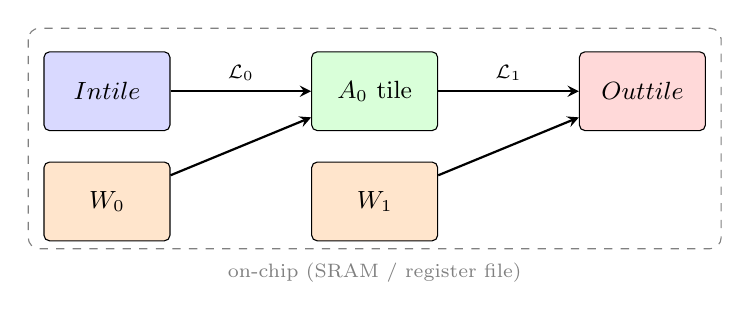
\begin{tikzpicture}[
    tile/.style={draw, minimum width=1.6cm, minimum height=1.0cm,
                 rounded corners=2pt, font=\small},
    arr/.style={->, >=stealth, thick}
  ]
  % Layer 0
  \node[tile, fill=blue!15] (in) at (0,0) {$\text{In tile}$};
  \node[tile, fill=orange!20] (w0) at (0,-1.4) {$W_0$};
  % Layer 0 output = intermediate
  \node[tile, fill=green!15] (a0) at (3.4,0) {$A_0$ tile};
  % Layer 1
  \node[tile, fill=orange!20] (w1) at (3.4,-1.4) {$W_1$};
  % Layer 1 output
  \node[tile, fill=red!15] (out) at (6.8,0) {$\text{Out tile}$};

  \draw[arr] (in) -- node[above, font=\scriptsize]{$\mathcal{L}_0$} (a0);
  \draw[arr] (w0) -- (a0);
  \draw[arr] (a0) -- node[above, font=\scriptsize]{$\mathcal{L}_1$} (out);
  \draw[arr] (w1) -- (out);

  % On-chip annotation
  \draw[dashed, gray, rounded corners=4pt]
    (-1.0, 0.8) rectangle (7.8, -2.0);
  \node[gray, font=\scriptsize] at (3.4, -2.3) {on-chip (SRAM / register file)};
\end{tikzpicture}
\caption{Fused execution of two consecutive layers.  The intermediate
  activation~$A_0$ is produced and consumed on-chip; only the network's
  input, weights, and final output cross the DRAM boundary.}
\label{fig:fused-two-layers}
\end{figure}

Consider fusing two convolutional layers with filter sizes
$R_0\!\times\!S_0$ and $R_1\!\times\!S_1$ respectively.
If the second layer requires an output tile of size $P\!\times\!Q$, it
needs an intermediate tile of size
$(P+R_1-1)\times(Q+S_1-1)$ from the first layer's output
(cf.\ the halo discussion in Section~\ref{sec:loop-ordering}).
To produce that intermediate tile, the first layer in turn needs an input
tile of size
\begin{equation}
\label{eq:fused-input-tile}
\bigl(P + R_1 - 1 + R_0 - 1\bigr) \times
\bigl(Q + S_1 - 1 + S_0 - 1\bigr).
\end{equation}
The tile sizes thus \emph{cascade backwards} through the fused layers,
and each intermediate tile is enlarged by its layer's corresponding
halo.  This cascading is precisely the phenomenon captured by
\emph{affine dimensions} (Definition~\ref{def:affine-dim} in
Section~\ref{sec:normal-affine}): the sums of indices (e.g.\ $p + r_1$
mapping to intermediate spatial positions) create dependencies that
propagate tile-size requirements across layers.

\paragraph{Memory-footprint implications.}
All intermediate tiles must fit simultaneously in an on-chip buffer,
since they are produced and consumed between consecutive loop
iterations without visiting DRAM.
Let $\text{FMEM}$ denote the on-chip feature memory.  In the two-layer
case the buffer must hold at least:
\begin{equation}
\label{eq:fused-footprint}
\text{footprint}
  \;\geq\;
  \underbrace{|I_{\text{tile}}|}_{\text{input tile}}
  +\;
  \underbrace{|A_{0,\text{tile}}|}_{\text{intermediate tile}}
  +\;
  \underbrace{|O_{\text{tile}}|}_{\text{output tile}}.
\end{equation}
As more layers are fused, additional intermediate tiles must be stored
concurrently, increasing the footprint.  Correspondingly, the output
tile size $P\!\times\!Q$ that fits within a given FMEM budget
\emph{decreases} with the number of fused layers, which can impact
data reuse and, in turn, energy efficiency.

% ------------------------------------------------------------------
\subsection{Multi-Layer Workload Formalization}
\label{sec:multi-layer-workload}

Section~\ref{sec:bg-workloads} formalized a single-layer computation as a
loop nest with a coupling that maps dimensions to operands.
Fusion extends this formalization: a fused group of $F$ layers is
expressed as a \emph{single, unified loop nest} whose coupling now defines
five categories of operands instead of three:
\begin{enumerate}
  \item \textbf{Input} (\texttt{in})—read-only tensor consumed by the
        first layer.
  \item \textbf{Weights} (\texttt{w})—one per layer ($W_0, \dots, W_{F-1}$),
        each referenced only by its own layer's dimensions.
  \item \textbf{Intermediate output} (\texttt{int\_out})—the output
        produced by every layer except the last; for layer~$i$ this is
        $A_i$.
  \item \textbf{Intermediate input} (\texttt{int\_in})—the input consumed
        by every layer except the first; layer~$i$ reads $A_{i-1}$, which
        is the \texttt{int\_out} of the previous layer.
  \item \textbf{Output} (\texttt{out})—write-only tensor produced by the
        last layer.
\end{enumerate}

In the Extended Einsum Notation (Section~\ref{sec:een}), a two-layer
fused convolution is written as:
\begin{align}
\label{eq:een-fused-2layer}
A_0[z_0, y_0, x_0] &\mathrel{+}= W_0[z_0, c_0, r_0, s_0]
  \cdot \text{In}[c_0, y_0\!+\!r_0, x_0\!+\!s_0], \notag\\[2pt]
\text{Out}[z_1, p, q] &\mathrel{+}= W_1[z_1, c_1, r_1, s_1]
  \cdot A_0[c_1, p\!+\!r_1, q\!+\!s_1].
\end{align}
All twelve dimensions ($C_0, Y_0, X_0, R_0, S_0, Z_0, C_1, R_1,
S_1, Z_1, P, Q$) appear in a single combined loop nest.  The coupling
tables for the five operand categories fully specify which dimensions
index which tensors (cf.\ Table~\ref{tab:coupling-conv} extended to
multiple layers).

This unified representation has two important consequences:
\begin{itemize}
  \item The \textbf{map space grows combinatorially} with the number of
        fused layers, because there are more dimensions, more factors, and
        more permutations.  The formula developed in
        Section~\ref{sec:bg-mapspace} applies unchanged, but
        $|\text{dims}|$ and $|\text{levels}|$ increase substantially:
        for an 11-layer fusion on a four-level hierarchy, the map space
        can exceed $10^{70}$, making exhaustive search intractable.
  \item The \textbf{cost model} must track per-layer MOPs for each
        intermediate tensor, respecting the producer--consumer chain and
        the cascading tile-size dependencies discussed above.
        Section~\ref{sec:bg-cost-model} generalizes naturally: reads and
        writes for \texttt{int\_in} and \texttt{int\_out} are computed
        per layer and weighted by the corresponding level's access energy,
        just as for \texttt{in}, \texttt{w}, and \texttt{out}.
\end{itemize}

% ------------------------------------------------------------------
\subsection{Inter-Layer vs.\ Intra-Layer Reuse}
\label{sec:inter-intra-reuse}

Two complementary forms of data reuse arise in fused execution:

\begin{description}
  \item[Intra-layer reuse]
    is the reuse discussed in Section~\ref{sec:data-reuse}:
    stationarity, halo overlap, and spatial multicast within a single
    layer.  These mechanisms remain available inside each fused layer and
    are optimized through tiling, loop ordering, and spatial unrolling
    exactly as for a single-layer mapping.

  \item[Inter-layer reuse]
    is unique to fusion.
    When intermediate activations reside on-chip, successive iterations
    of the \emph{outer} (consuming) layer can reuse portions of the
    intermediate tile that were produced by a previous iteration of the
    \emph{inner} (producing) layer, provided the halo regions overlap.
    The amount of inter-layer reuse depends on the relative tile sizes,
    filter dimensions, and loop ordering across layers.
\end{description}

The total on-chip reuse in a fused mapping is the combination of both
forms.  A good mapper must balance them: aggressively tiling the
intermediate tensor to maximize inter-layer reuse can starve intra-layer
reuse within each individual layer, and vice versa.

% ------------------------------------------------------------------
\subsection{Choosing Which Layers to Fuse}
\label{sec:fusion-choices}

Not all layers benefit equally from fusion.  The decision of which
consecutive layers to group into a fused set depends on several factors:

\begin{itemize}
  \item \textbf{On-chip memory budget.}
        Each additional fused layer increases the memory footprint
        (Equation~\eqref{eq:fused-footprint}).  If the on-chip buffer
        cannot accommodate the combined intermediate tiles, the output
        tile must shrink, reducing data reuse and potentially increasing
        total energy.

  \item \textbf{Intermediate activation volume.}
        Fusion is most beneficial when the intermediate tensors are
        large—i.e.\ when the spatial resolution is high and the number
        of channels is moderate.  This corresponds to the
        \emph{activation-dominant} regime described in
        Section~\ref{sec:act-weight-dominant}.  Conversely, fusing
        layers in the \emph{weight-dominant} regime (deep layers with
        many channels and small spatial dimensions) yields diminishing
        returns because the intermediate traffic is already small.

  \item \textbf{Compatibility constraints.}
        Certain layer types (e.g.\ pooling, batch normalization, skip
        connections, element-wise activations) interact with the
        producer--consumer chain.
        Element-wise operations such as ReLU are trivially fused because
        they do not alter the tensor shape.
        Pooling layers reduce spatial dimensions and must be accounted for
        when propagating tile sizes backward.
        Skip connections break the strictly sequential chain and require
        additional buffer capacity to hold the ``shortcut'' tensor until
        it is needed.

  \item \textbf{Diminishing returns.}
        Beyond a certain depth of fusion, the marginal DRAM traffic saved
        by adding one more layer decreases while the memory pressure on
        the on-chip buffer and the map-space size continue to grow.
        Finding the optimal \emph{fusion depth}—that is, how many
        layers to fuse together—is itself a combinatorial problem.
\end{itemize}

Several works have addressed the fusion-set selection problem.
\textbf{Alwani et~al.}~\cite{alwani2016fused} first demonstrated
fused-layer CNN accelerators, proposing a greedy algorithm that fuses
consecutive layers while the intermediate tiles fit in on-chip memory.
\textbf{Xiao et~al.}~\cite{xiao2017exploring} extended this analysis
by exploring the trade-off between fusion depth and output tile size.
\textbf{Tangram}~\cite{gao2019tangram} introduced a
\emph{set-based} partitioning of the dataflow graph, allowing non-contiguous
and parallel fusion sets.
\textbf{Optimus}~\cite{li2023optimus} formulates the partition into fusion
sets as an optimization problem solved by dynamic programming.
\textbf{Herald}~\cite{kwon2023herald} proposes a heterogeneous
dataflow that dynamically switches between layer-by-layer and fused
execution depending on on-chip resource availability.

In this thesis, the focus is on the \emph{mapping} of an already-determined
fusion set rather than on the selection of which layers to fuse.
The analytical cost model and mapper developed in the following chapters
accept any fusion depth and optimize the combined loop nest accordingly,
enabling systematic evaluation of both shallow and deep fusion
configurations.

% ------------------------------------------------------------------
\subsection{Summary}
\label{sec:fusion-summary}

Layer fusion eliminates the dominant source of DRAM traffic in DNN
inference—intermediate activations—by keeping them on-chip across
consecutive layers.
Its effectiveness hinges on three aspects: (i)~the cascading tile-size
dependencies that arise from producer--consumer relationships,
(ii)~the interplay between inter-layer and intra-layer reuse, and
(iii)~the memory-footprint constraints of the on-chip buffer.
Formally, fusion extends the single-layer loop nest and coupling into a
unified multi-layer formulation with five operand categories, enlarging
both the cost model and the map space.
The following chapters build on this foundation to present the
FactorFlow framework extended with native layer-fusion support.
   % 2.7  Layer Fusion
